\section{Ziel}
Bestimmung der Brennweite verschiedener Linsen und Linsensysteme.
\section{Theorie}
Linsen brechen das Licht aufgrund von Ein-/ bzw Austritt aus dem Linsenmedium welches optisch dichter ist.
Generell unterschiedet man zwei Typen von Linsen
\subsection{Die Linsentypen}
\subsubsection*{Sammellinsen}
Sammellinsen werden zum Linsenrand dünner und bündeln somit paralles Licht im sogenannten Brennpunkt.
Die Brennweite $f$ und die Bildweite $b$ sind dabei stehts positiv.
Man spricht somit von einem rellen Bild was entsteht.
\begin{figure}[H]
    \centering
    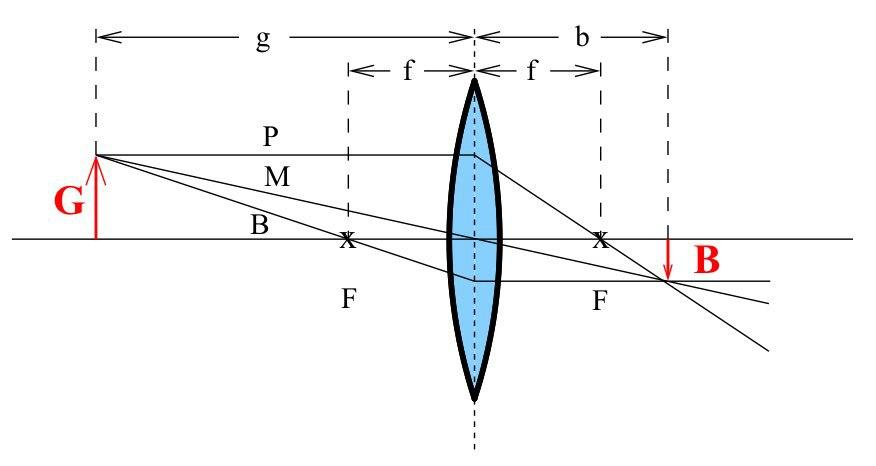
\includegraphics[width=0.6\textwidth]{bilder/sammellinse.jpg}
    \caption{Darstellung der Bildkonstruktion einer Sammellinse mit der Bildgröße $B$,
    Gegenstandsgröße $G$, Brennpunkt $F$, Brennweite $f$ und Bildweite $b$.\cite[1]{anleitung}}
\end{figure}

\subsubsection*{Zerstreuungslinse}
Die Zerstreuungslinse wird, im Gegensatz zu Sammellinse, zum Linsenrand hin dicker.
Ihre Brennweite $f$ und Bildweite $b$ sind negativ. Man spricht von einem virtuellen Bild was entsteht.
\begin{figure}[H]
    \centering
    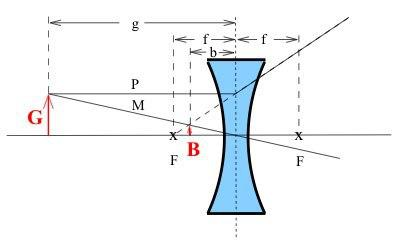
\includegraphics[width=0.6\textwidth]{bilder/zerlinse.jpg}
    \caption{Darstellung der Bildkonstruktion einer Zerstreuungslinse mit der Bildgröße $B$,
    Gegenstandsgröße $G$, Brennpunkt $F$, Brennweite $f$ und Bildweite $b$.\cite[1]{anleitung}}
\end{figure}

Bei den, wie oben angesprochenen, Linsen mit spricht man von dünnen Linsen, sie besitzen eine
Hauptebene an dem das Licht gebrochen wird.\\
Werden die Linsen dicker, so reicht diese beschreibung mit einer Hauptebenen nicht mehr aus. Es benötigt zwei Hauptebenen, an 
denen man sich die Lichtstrahlen gebrochen denkt.
\begin{figure}
    \centering
    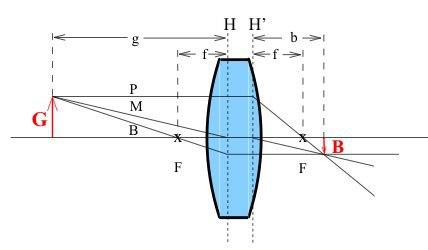
\includegraphics[width=0.6\textwidth]{bilder/dickelinse.jpg}
    \caption{Darstellung einer dicken Sammellinse mit zwei eingezeichneten Hauptebenen.\cite[1]{anleitung}}
\end{figure}
\subsection{Bildkonstruktion}
Für die Bildkonstruktion betrachte man die drei ausgezeichneten Strahlen.
\begin{enumerate}
    \item Parallelstrahl $P$\\
    Er verläuft parallel vom Gegenstand zur optischen Achse und wird an der Mittelebene der Linse gebrochen.
    \item Mittelpunktstrahl $M$\\
    Er verläuft durch die Mitte der Linse und ändert somit seine Richtung nicht.
    \item Brennpunktstrahl $B$\\
    Er verläuft durch den Brennpunkt der Linse und wird zum Parallelstrahl hin gebrochen.
\end{enumerate}
Aus den Strahlensätzen folgt damit:
\begin{equation}
    V=\frac{B}{G}=\frac{b}{g}.
    \label{eqn:strahl}
\end{equation}
Mit der Bildgröße $B$, Gegenstandsgröße $G$, Bildweite $b$ und Gegenstandsweite $g$.
Sowie die Linsengleichung
\begin{equation}
    \frac{1}{f}=\frac{1}{b}+\frac{1}{g}.
    \label{eqn:linsengl}
\end{equation}

Streng genommen gelten Gl. \ref{eqn:strahl}, \ref{eqn:linsengl} nur für achsennahe Strahlen, da achsenferne Strahlen
stärker gebrochen werden und es somit zu Abbildungsfehler (unscharfes Bild) kommen kann.
Für zusammengesetzte Linsen (Linsensysteme) addieren sich die rezipoken Brennweiten und definieren die Brechkraft
\begin{equation}
    D=\sum_i^N D_i
\end{equation}
\label{sec:Theorie}
